\section{تولید دادگان ترکیبی و آموزش مدل تشخیص خودرو و تایر}

در این بخش از تمرین، هدف ایجاد یک مدل یکپارچه است که بتواند به طور همزمان «خودرو» و «تایر» را در تصویر تشخیص دهد. از آنجا که پایگاه داده‌ی اولیه‌ی ما تنها شامل برچسب‌های تایر بود، از تکنیک برچسب‌گذاری خودکار (\lr{Auto-Labeling}) به کمک یک مدل از پیش‌آموزش‌دیده برای استخراج کادرهای خودرو استفاده کردیم.

\subsection{تولید برچسب‌های ترکیبی (\lr{Auto-Labeling})}

برای جلوگیری از برچسب‌زنی دستیِ هزاران تصویر، مدل پایه‌ی \lr{YOLOv8n} (که روی دادگان \lr{COCO} آموزش دیده و قادر به تشخیص خودرو به عنوان کلاس ۲ است) بر روی تصاویر اعمال شد. خروجی این مدل با برچسب‌های موجودِ تایر ترکیب شده و فایل‌های متنی جدیدی تولید گردید.

\begin{codebox}[\lr{Auto-Labeling Logic}]
\begin{lstlisting}[language=Python]
# car_model: Pre-trained YOLOv8n
# img_path: Path to the current image in the dataset

results = car_model.predict(img_path, classes=[2], verbose=False)
car_lines = []
h, w = img.shape[:2]

for r in results:
    if r.boxes is not None:
        for box in r.boxes:
            x1, y1, x2, y2 = map(float, box.xyxy[0])
            cx = ((x1 + x2) / 2) / w
            cy = ((y1 + y2) / 2) / h
            bw = (x2 - x1) / w
            bh = (y2 - y1) / h
            # Assigning Class '0' for Car
            car_lines.append(f"0 {cx:.6f} {cy:.6f} {bw:.6f} {bh:.6f}\n")

# car_lines are then appended to the existing tyre labels (Class '1')
\end{lstlisting}
\end{codebox}

\begin{notebox}[مزیت این رویکرد]
تکنیک \lr{Auto-Labeling} یا \lr{Pseudo-Labeling} در پروژه‌های صنعتی به شدت کاربرد دارد. این روش زمان آماده‌سازی داده را به حداقل رسانده و به ما اجازه می‌دهد از دانشِ مدل‌های قدرتمند قبلی (مانند \lr{COCO}) برای توسعه‌ی مدل‌های تخصصیِ چندکلاسه استفاده کنیم.
\end{notebox}

\subsection{آموزش شبکه‌ی یکپارچه}

پس از ایجاد فایل‌های متنی حاوی هر دو کلاس (۰: خودرو، ۱: تایر)، فایل پیکربندی \lr{YAML} ساخته شده و مدل جدید از صفر بر روی این مجموعه‌ی غنی‌شده به مدت ۱۵ دور (\lr{Epoch}) آموزش داده شد.

\begin{codebox}[\lr{Training the Combined Model}]
\begin{lstlisting}[language=Python]
data_config = {
    'path': '/content/car_tyre_dataset',
    'train': 'train/images',
    'val': 'valid/images',
    'nc': 2,
    'names': {0: 'car', 1: 'tyre'}
}

model_combined = YOLO("yolov8n.pt") 
results = model_combined.train(data="dataset.yaml", epochs=15, imgsz=640)
\end{lstlisting}
\end{codebox}

\subsection{تحلیل کمی: ارزیابی نمودارهای آموزش}

پس از ۱۵ دور آموزش، توابع هزینه و معیارهای دقت شبکه استخراج شدند تا رفتار مدل در طول فرآیند بهینه‌سازی تحلیل شود.

\begin{figure}[h!]
    \centering
    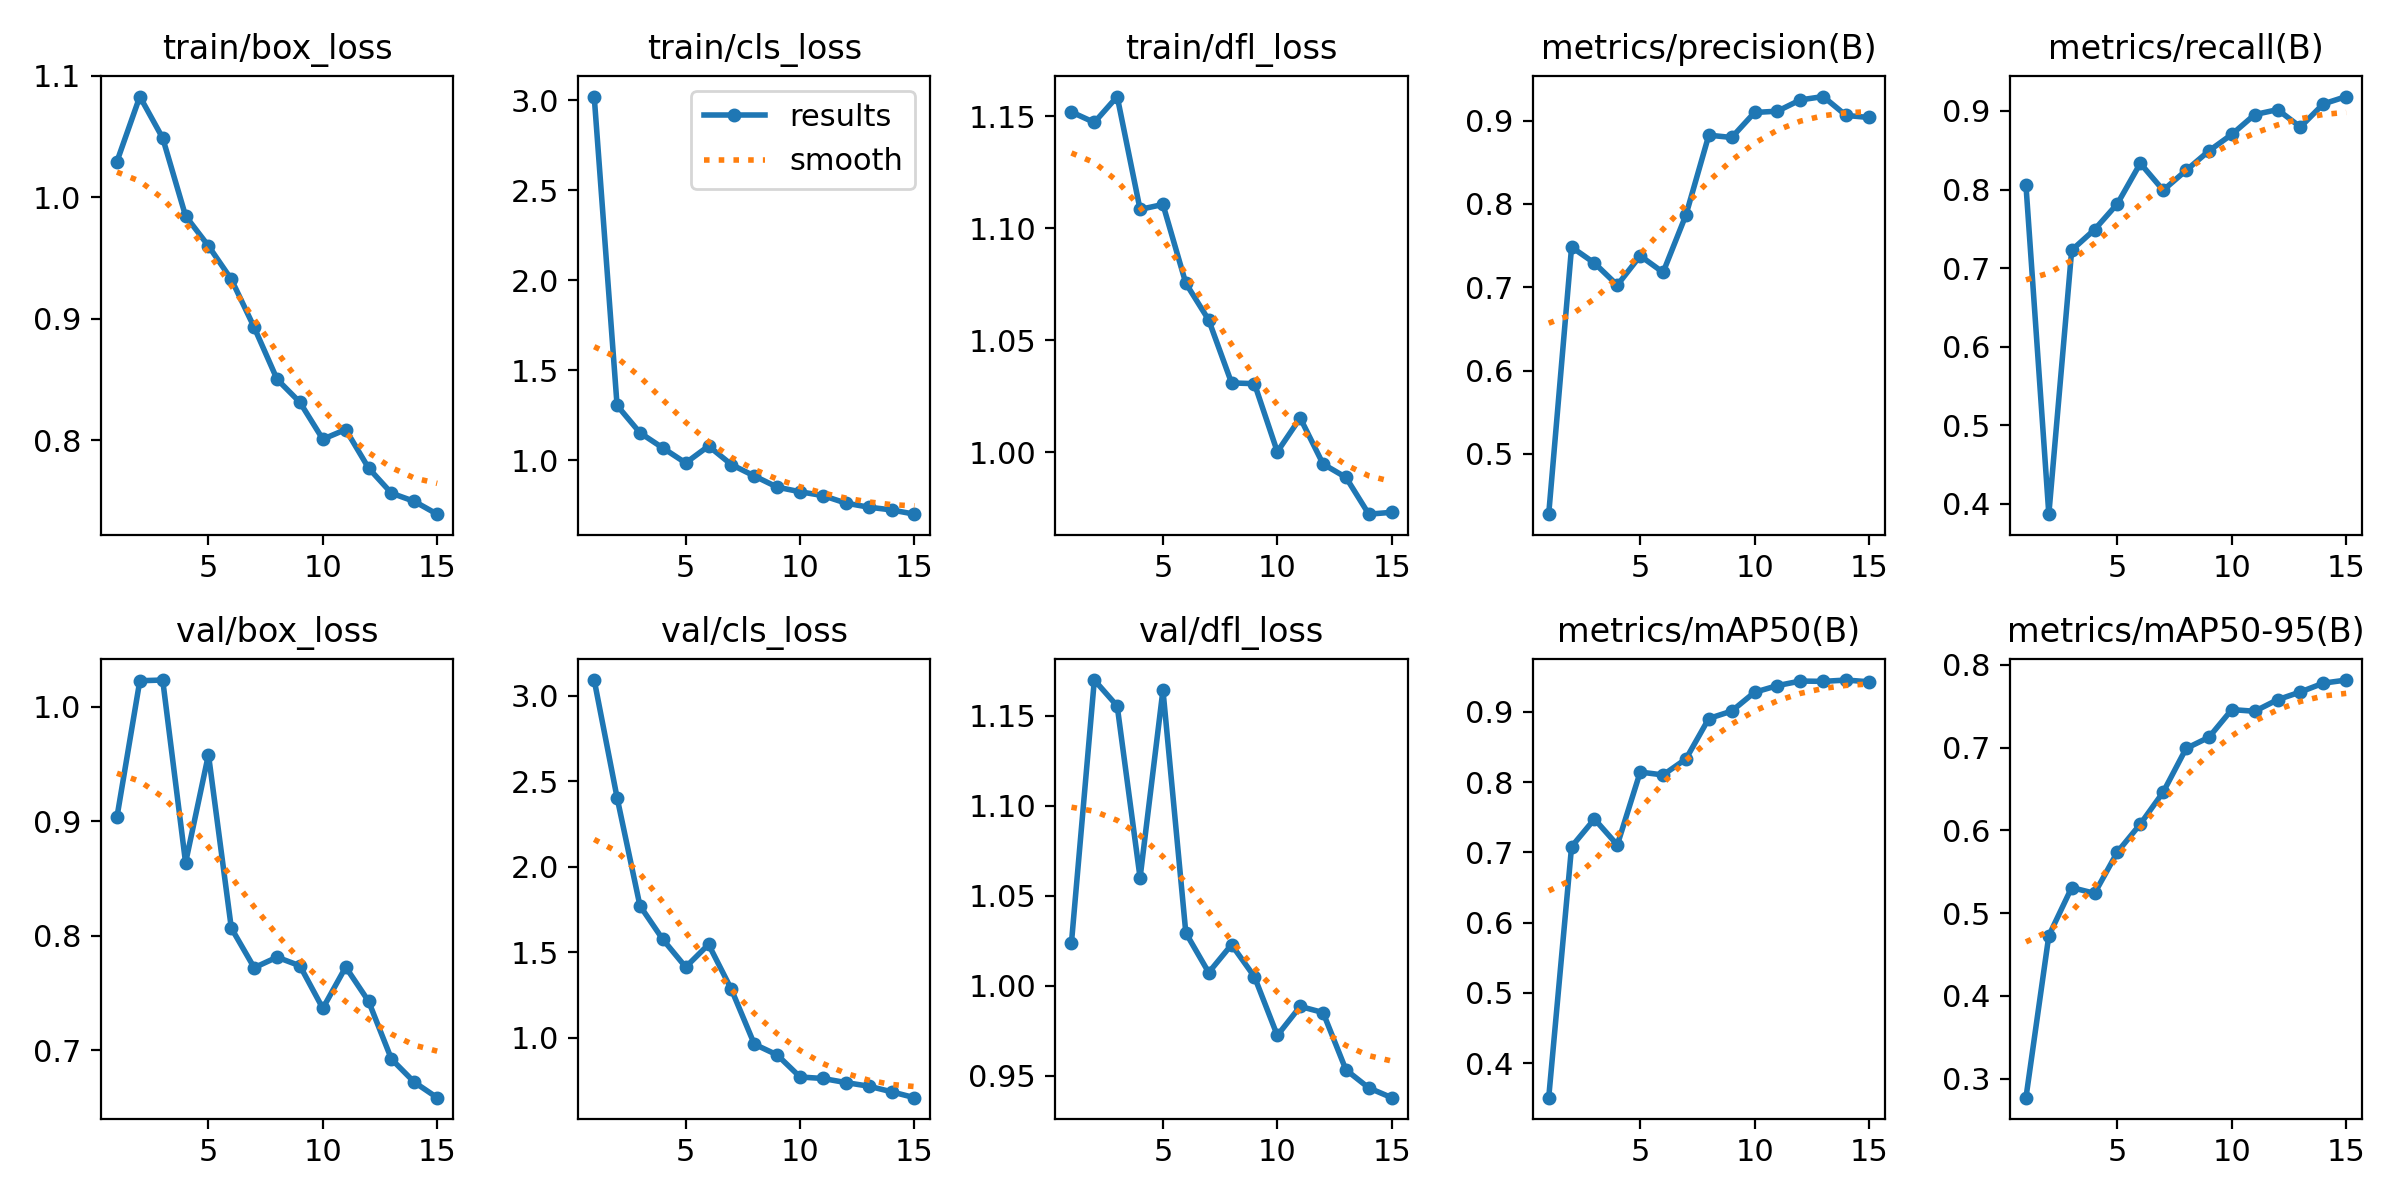
\includegraphics[width=\textwidth]{loss_map_car_tyre.png}
    \caption{روند آموزش مدل ترکیبی خودرو و تایر طی ۱۵ دور (\lr{Epoch})}
    \label{fig:loss_car_tyre}
\end{figure}

\newpage
با تحلیل نمودارهای شکل \ref{fig:loss_car_tyre}، نکات مهندسی زیر استخراج می‌شود:
\begin{itemize}
    \item \textbf{یادگیری سریع کلاس‌ها (\lr{cls\_loss}):} نمودار خطای دسته‌بندی با یک شیب بسیار تند در همان ۳ دور اول افت کرده است. این نشان می‌دهد که تفاوت ظاهری بین «خودرو» و «تایر» برای شبکه بسیار واضح بوده و مدل خیلی سریع توانسته ویژگی‌های متمایزکننده‌ی این دو کلاس را یاد بگیرد.
    \item \textbf{تثبیت خطای کادر (\lr{box\_loss}):} برخلاف خطای دسته‌بندی، خطای مختصات کادر با شیب ملایم‌تری کاهش یافته است. وجود کمی نوسان در نمودار \lr{val/box\_loss} طبیعی است، زیرا مدل در حال تنظیم دقیق ابعاد کادرهای تایر است که به دلیل تنوع زوایا و سایه‌ها چالش‌برانگیزتر است.
    \item \textbf{دقت فوق‌العاده (\lr{mAP50}):} رسیدن به دقت بالای ۹۰ درصد (بالای ۰.۹) در تنها ۱۵ دور، موفقیت‌آمیز بودن استراتژی \lr{Auto-Labeling} ما را تضمین می‌کند. داده‌های تولید شده به قدری تمیز بوده‌اند که مدل توانسته به سرعت روی آن‌ها همگرا شود.
\end{itemize}

\subsection{تحلیل کیفی: بررسی چالش‌های تشخیص در شرایط واقعی}

برای درک بهتر عملکرد شبکه، مدل یکپارچه بر روی نمونه‌هایی از داده‌های ارزیابی تست شد. در این تصاویر، خودروها با کادر سبز و تایرها با کادر آبی مشخص شده‌اند.

\begin{figure}[h!]
    \centering
    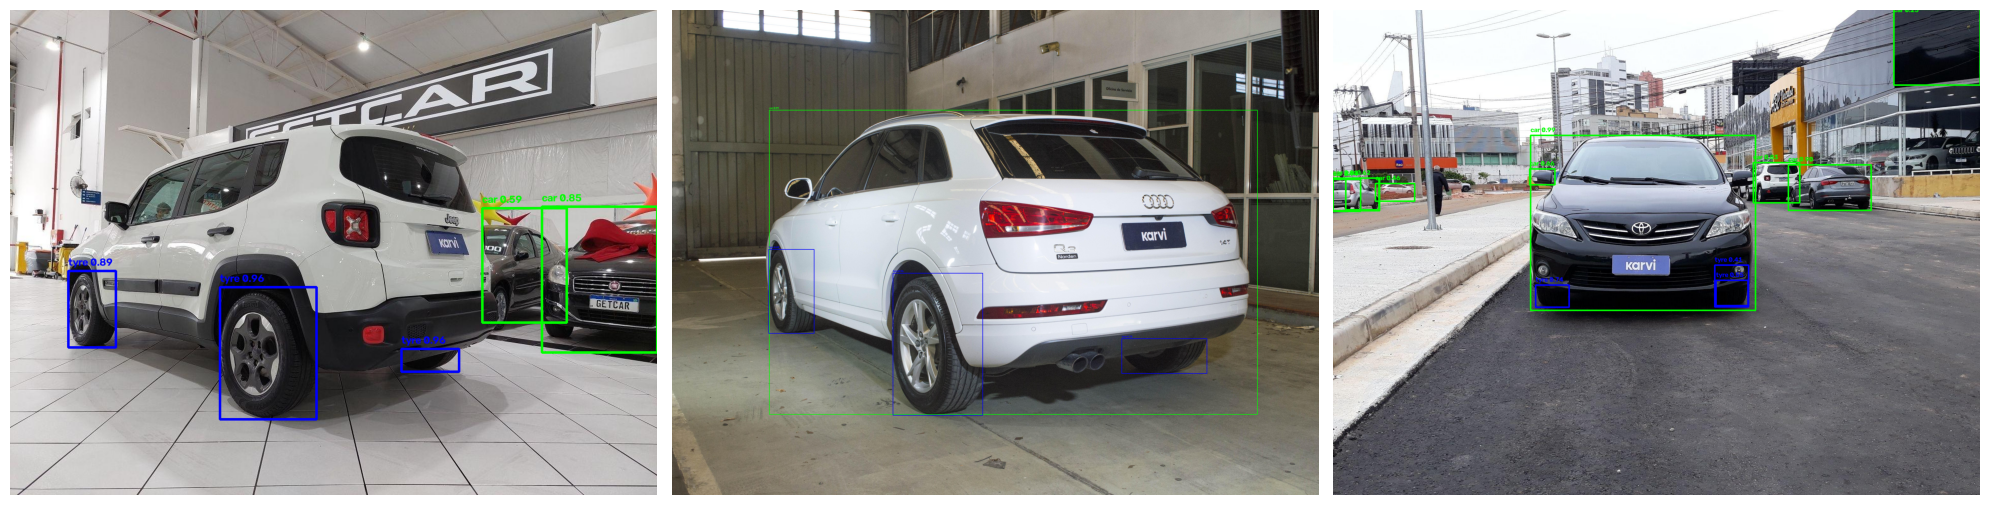
\includegraphics[width=\textwidth]{sample_cars.png}
    \caption{نمونه خروجی مدل ترکیبی. رنگ سبز: خودرو، رنگ آبی: تایر}
    \label{fig:sample_cars}
\end{figure}

بررسی دقیق تصاویر در شکل \ref{fig:sample_cars} نقاط قوت و همچنین ضعف‌های ظریف مدل را آشکار می‌کند:
\begin{itemize}
    \item \textbf{تشخیص پایدارِ خودروها:} در تمامی تصاویر، مدل توانسته خودروی اصلی و حتی خودروهای موجود در پس‌زمینه (تصویر اول و سوم) را با دقت بالا (کادرهای سبز) تشخیص دهد. هیچ خودرویی در میدان دید از دست نرفته است.
    \item \textbf{چالش انسداد و پرسپکتیو در تایرها:} در تصویر دوم (خودروی سفید میانی)، مدل به درستی تایرهای جلو و عقب سمتی که رو به دوربین است را تشخیص داده و حتی تایر سمت شاگرد را که نیمی از آن پنهان است به خوبی کادربندی کرده است.
    \item \textbf{تحلیل خطاهای مثبت کاذب (\lr{False Positives}):} با نگاهی مهندسی به خروجی‌ها، متوجه خطاهای جالبی در تشخیص تایر (کادرهای آبی) می‌شویم:
    \begin{itemize}
        \item در تصویر اول و دوم، بخش‌هایی از سیستم اگزوز یا سایه‌های تیره در زیر سپر عقب به عنوان تایر تشخیص داده شده‌اند.
        \item در تصویر سوم (خودروی مشکی رنگ)، قاب‌های مه‌شکنِ روی سپر جلو به دلیل فرم دایره‌ای و تیره‌رنگ بودن، شباهت بصری زیادی به تایر داشته و مدل به اشتباه آن‌ها را تایر تشخیص داده است.
    \end{itemize}
\end{itemize}

\begin{tipbox}[راه‌حل برای بهبود خطاهای مدل]
بروز چنین خطاهایی در شبکه‌های \lr{CNN} به این دلیل است که مدل در حال حاضر تنها به ویژگی‌های محلی (رنگ تیره و فرم دایره‌ای) توجه می‌کند. برای رفع این مشکل، می‌توان در دوره‌های بعدی آموزش از تکنیک \lr{Data Augmentation} هدفمند (تغییر روشنایی قسمت‌های پایینی تصویر) استفاده کرد یا نمونه‌های منفی (\lr{Background Images}) شامل سپرهای ماشین بدون تایر را به دادگان اضافه نمود تا مدل یاد بگیرد هر دایره‌ی تیره‌ای لزوماً تایر نیست.
\end{tipbox}